% \documentclass[notes=onlyslideswithnotes]{beamer}
\documentclass{beamer}


\usepackage[no-math]{fontspec}
\usepackage{xunicode}
\usepackage{xltxtra}
\usepackage{tikz}
\usepackage{graphicx}
\usepackage{booktabs}
\usepackage{fontawesome}
\usepackage[normalem]{ulem}
\usepackage[mode=text]{siunitx}
\usepackage{hyperref}


% Beamer setup
\mode<presentation>
{
	\usetheme{OtagoPlain}
	\setbeamertemplate{navigation symbols}{}
    \setbeamertemplate{title in head/foot}{Mining decision-making processes in OSSD: Python PEPs}
    % \insertshorttitle comes out alerted for some reason and I don’t have time to figure out why
}
 

% TikZ setup
\usetikzlibrary{positioning}
\usetikzlibrary{calc}
\usetikzlibrary{arrows.meta}
\usetikzlibrary{shapes.geometric}


% fontspec setup
\defaultfontfeatures{Mapping=tex-text}
\setmainfont{Minion Pro}
\setsansfont[Scale=MatchUppercase,BoldFont={Open Sans}]{Open Sans Light}
\setmonofont[Scale=MatchLowercase]{Iosevka Light}


% graphicx setup
\graphicspath{{images/}}


% misc
\newcommand{\todo}[1]{\alert{\textbf{!!TODO!! [#1] !!}}}


% Draw a grid to aid TikZ picture drawing/debugging.
\newcommand{\DrawGridTikZ}[2]{%
	\begin{scope}[color=lightgray]
		\draw[thin,step=1mm]  (0.0,0.0)   grid (#1,#2);%
		\draw[thick,step=1cm] (-0.1,-0.1) grid (#1+0.1,#2+0.1);%
		\pgftext[top,at={\pgfxy(0.0,-0.2)}]{\tiny 0}%
		\pgftext[right,at={\pgfxy(-0.2,0.0)}]{\tiny 0}%
		\foreach \x in {1,...,#1} {\pgftext[top,at={\pgfxy(\x,-0.2)}]{\tiny\x}}%
		\foreach \y in {1,...,#2} {\pgftext[right,at={\pgfxy(-0.2,\y)}]{\tiny\y}}%
	\end{scope}
}


% Sometimes we want to put a comment in tiny text on the next line, but the default line skip
% will insert too much vertical space. Put a \tinyskip at the end of the line instead.
\def\tinyskip{\\[-0.33\baselineskip]}


% Increase item separation of level 1 list items. Can't use enumitem because it breaks beamer lists :(.
% See: <https://tex.stackexchange.com/a/31524>
\makeatletter
\patchcmd{\@listI}{\itemsep3\p@}{\itemsep6\p@}{}{}
\makeatother


% Bold-face text using the structure colour.
\newcommand<>{\structurebf}[1]{\structure#2{\textbf{#1}}}
\newcommand<>{\alertbf}[1]{\alert#2{\textbf{#1}}}


% preamble
\title{Mining decision-making processes in \\ Open Source software development}
\subtitle{A study of Python Enhancement \\ Proposals (PEPs) using email repositories}
\author{Nigel Stanger}
\date{May 1, 2020}


\begin{document}


%%%%%%%%%%%%%%%%%%%%%%%%%%%%%%%%%%%%%%%%%%%%%%%%%%%%%%%%%%%%%%%%%%%%%%%%%%%%%%%%


% \setbeamertemplate{background canvas}{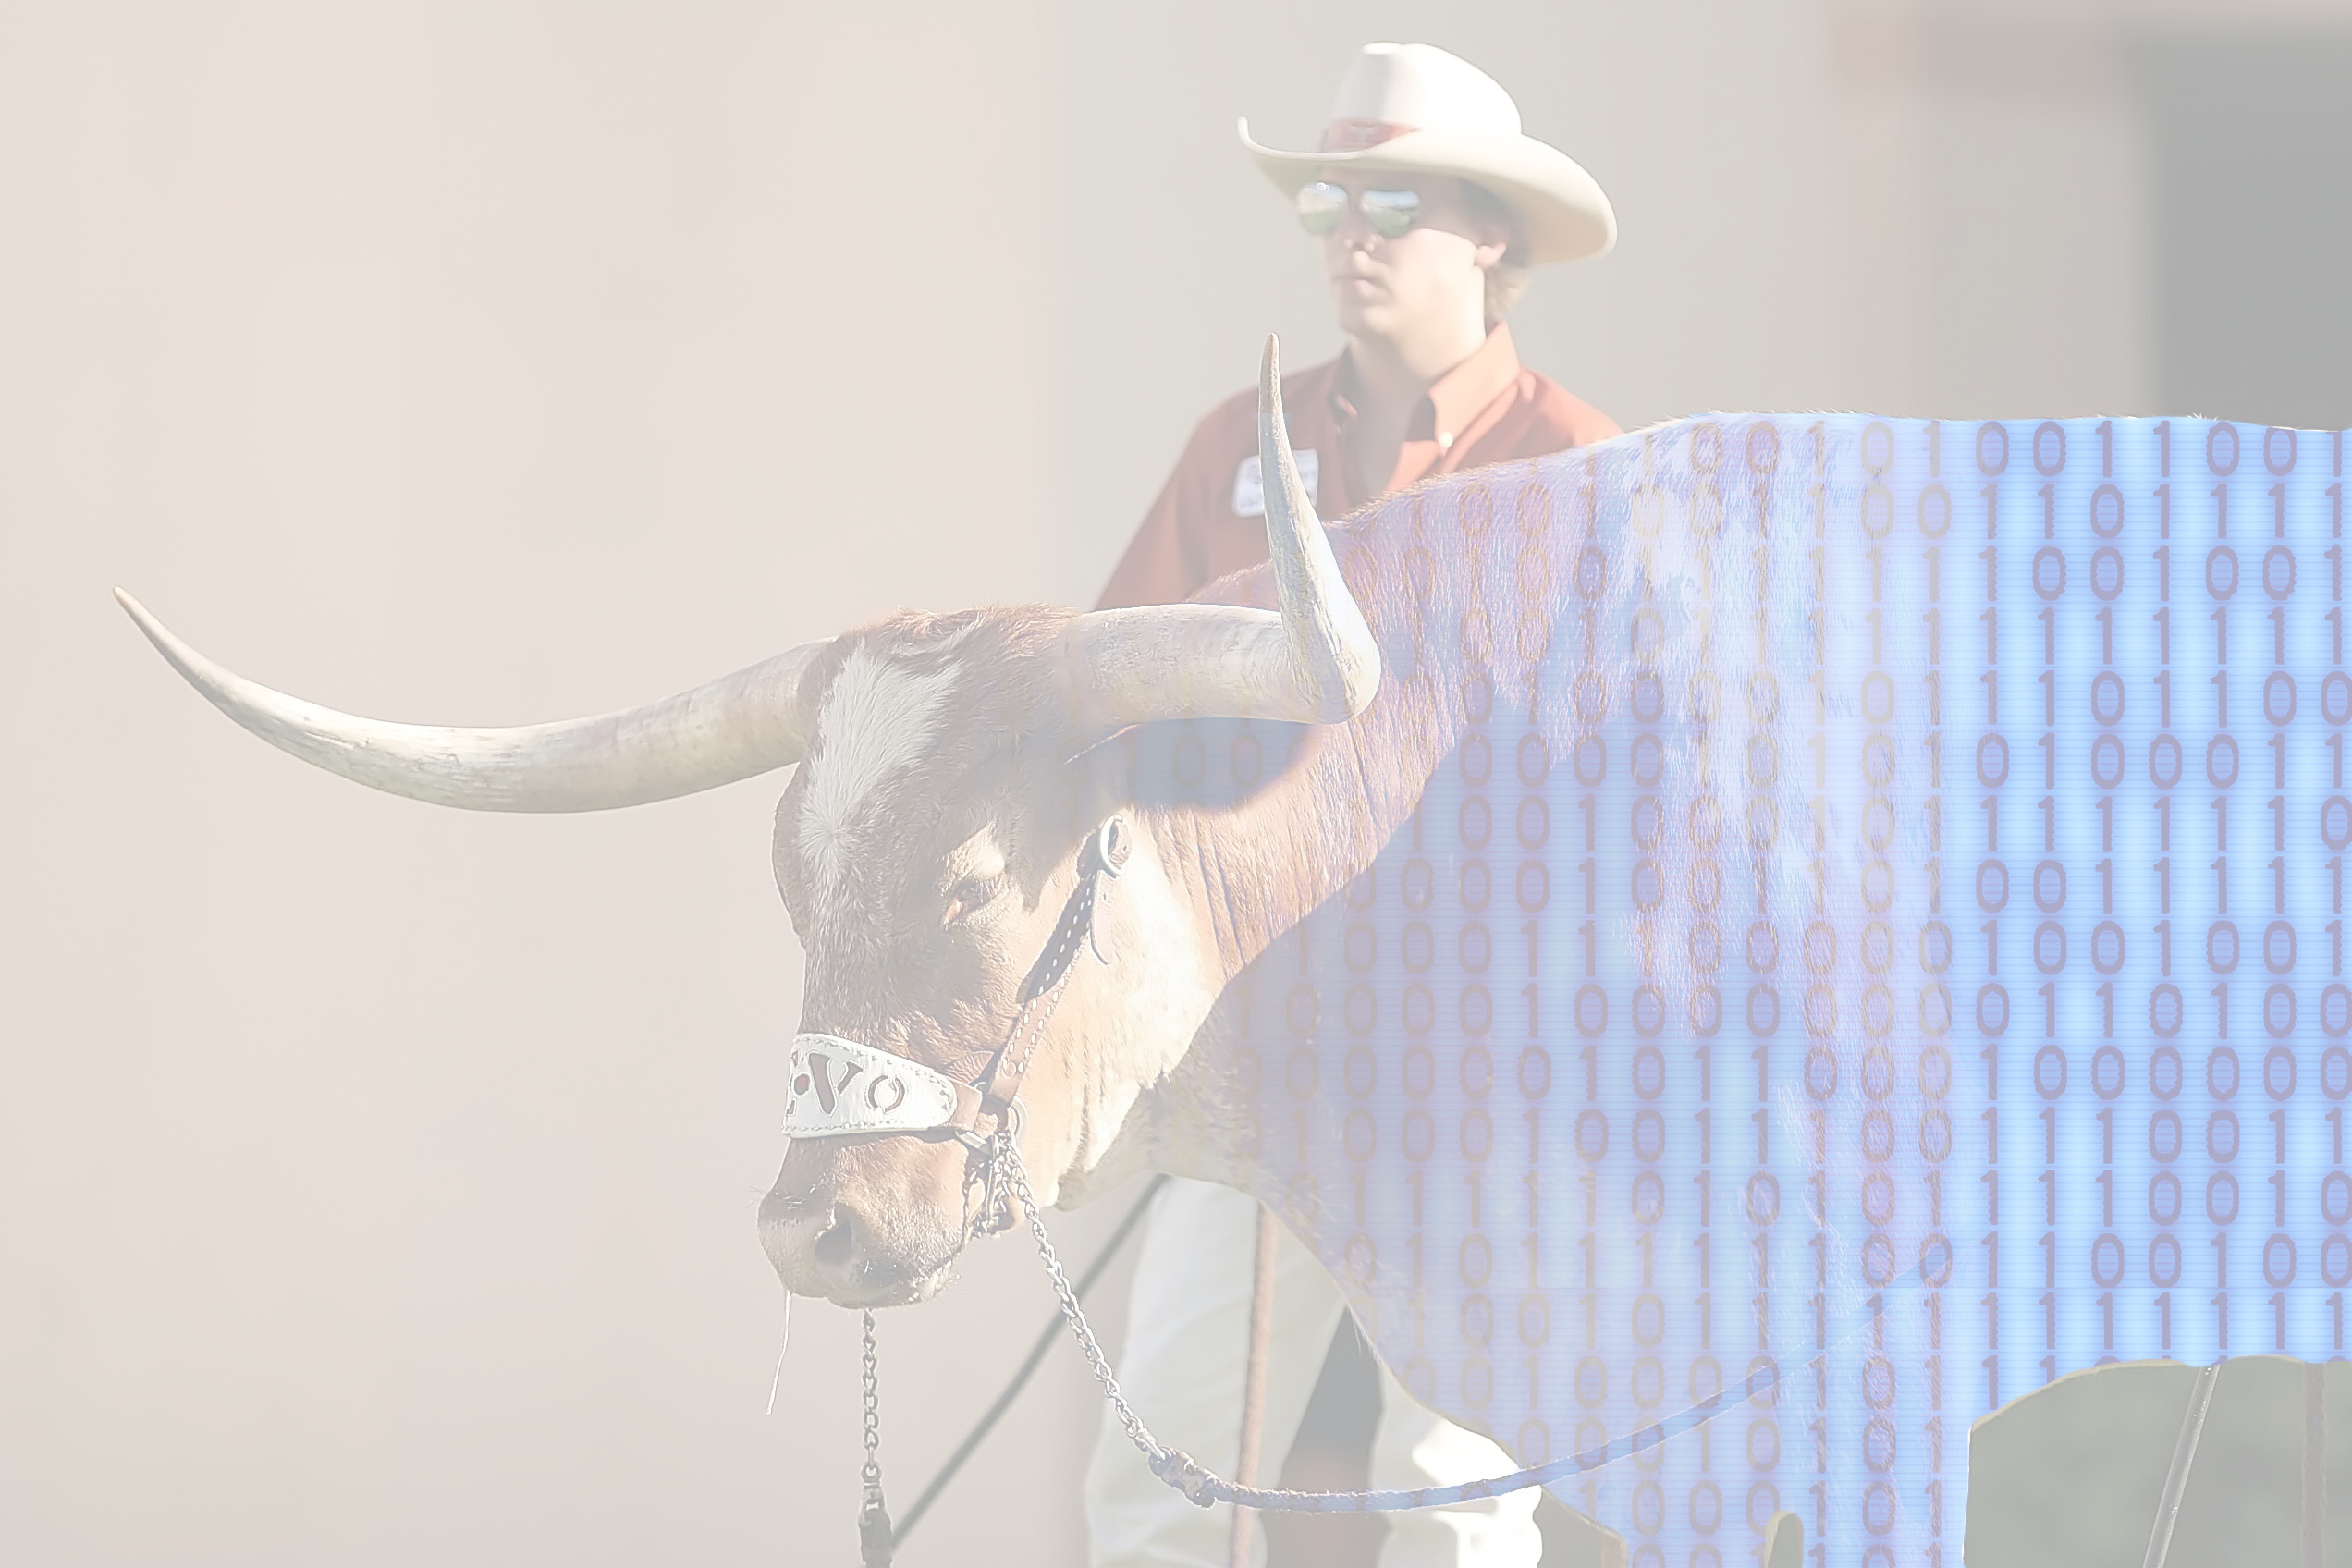
\includegraphics[height=\paperheight,keepaspectratio]{data-wrangler-BG.jpg}}
% to create image:
%   1. export data-wrangler.xcf as PNG from GIMP
%   2. convert data-wrangler.png -fill white -colorize 67% data-wrangler-BG.jpg

\begin{frame}
    \thispagestyle{empty}
    \titlepage
\end{frame}

% \setbeamertemplate{background canvas}[default]


%%%%%%%%%%%%%%%%%%%%%%%%%%%%%%%%%%%%%%%%%%%%%%%%%%%%%%%%%%%%%%%%%%%%%%%%%%%%%%%%


\begin{frame}
    \frametitle{What we did\footnote{Pankajeshwara Sharma, Bastin Tony Roy Savarimuthu, and Nigel Stanger. Mining decision-making processes in Open Source software development: A study of Python Enhancement Proposals (PEPs) using email repositories. In \emph{Proceedings of the 24th International Conference on Evaluation and Assessment in Software Engineering (EASE’20)}, pages 200–209. doi: 10.1145/3383219.3383240.}}

    \begin{itemize}
        \item Extracted the actual decision-making process used by the Python community to evolve the language:
        \begin{itemize}
            \item from the Python mailing list archives (≈1.5 million messages)
            \item compared it with previously documented processes
        \end{itemize}
        \item Focused on Python Enhancement Proposals (PEPs) as the primary decision-making framework.
    \end{itemize}
    \bigskip

    \structurebf{Why?} To gain deeper insights into the decision-making processes of Open Source software development communities—is what they say they do \emph{actually} what they do?
\end{frame}


%%%%%%%%%%%%%%%%%%%%%%%%%%%%%%%%%%%%%%%%%%%%%%%%%%%%%%%%%%%%%%%%%%%%%%%%%%%%%%%%


\begin{frame}
    \frametitle{OSS governance}

    \begin{itemize}
        \item Good governance is a key factor in successful OSS projects. \tinyskip
        {\tiny (O'Mahony \& Ferraro, 2007)}
        \begin{itemize}
            \item geographically dispersed
            \item diverse teams
            \item promotes good decision-making
        \end{itemize}
        \item Typical OSS governance models:
        \note[item]{There are some overlaps between these, of course.}
        \begin{itemize}
            \item hierarchical (e.g., Apache)
            \note[item]{Kind of a corporate model, with many levels, committees, etc.}
            \item community consensus (e.g., PostgreSQL)
            \item monarchist/dictatorship (e.g., Linux)
            \note[item]{One person makes the final decisions. I’m talking more about the Linux kernel here. Monarchist models have been studied less than the other two.}
        \end{itemize}
    \end{itemize}
\end{frame}


%%%%%%%%%%%%%%%%%%%%%%%%%%%%%%%%%%%%%%%%%%%%%%%%%%%%%%%%%%%%%%%%%%%%%%%%%%%%%%%%


\begin{frame}
    \frametitle{Decision-making processes}

    \begin{itemize}
        \item Having explicit decision-making processes can promote community cohesion and accountability, \structurebf{BUT}:
        \begin{itemize}
            \item processes often evolve over time
            \item[\(\Rightarrow\)] enacted process may not match advertised process
            \item community members may not be aware of this
            \note[item]{Especially new members.}
            \item evidence buried in reams of community discussion
            \note[item]{Mailing lists, discussion forums, IRC, …. Especially projects with a long history.}
        \end{itemize}
        \item Need to make the enacted process explicit.
        \begin{itemize}
            \item \alert{data-driven, bottom-up approach}
            \item data from project communication repositories {\tiny (e.g., mailing lists)}
        \end{itemize}
    \end{itemize}
\end{frame}


%%%%%%%%%%%%%%%%%%%%%%%%%%%%%%%%%%%%%%%%%%%%%%%%%%%%%%%%%%%%%%%%%%%%%%%%%%%%%%%%


\begin{frame}
    \frametitle{Why Python?}

    \begin{itemize}
        \item Well known OSS project with a long history (1990).
        \note[item]{Community discussion archives go back to 1999.}
        \item Well documented governance model and decision-making process. {\tiny (including change history)}
        \item Followed a monarchist model up to 2019.
        \note[item]{Monarchist models haven’t been all that well studied in the literature.}
        \begin{itemize}
            \item Guido van Rossum as \emph{Benevolent Dictator for Life (BDFL)}
            \item small “inner circle” of core developers
            \item BDFL or delegate made all final decisions
            \item Guido resigned July 2018 \(\Rightarrow\) steering council December 2018
            \note[item]{So most of the data covers the monarchist period before Guido resigned.}
        \end{itemize}
        \item Complete mailing list archives available. {\tiny (≈1.5 million messages over 20 years)}
        \item Prior work found their enacted process appeared to differ from the advertised process at a high level. \tinyskip
        {\tiny (Keertipati et al., 2017; Savarimuthu et al., 2016)}
    \end{itemize}
\end{frame}


%%%%%%%%%%%%%%%%%%%%%%%%%%%%%%%%%%%%%%%%%%%%%%%%%%%%%%%%%%%%%%%%%%%%%%%%%%%%%%%%


\begin{frame}
    \frametitle{The Python decision-making process}

    \begin{itemize}
        \item Centres around \emph{Python Enhancement Proposals (PEPs)}. {\tiny (cf.\ RFCs)}
        \begin{itemize}
            \item PEP 0 currently lists 515 {\tiny (\url{https://www.python.org/dev/peps/})}
            \item Process (44), Informational (83), Standards Track (388)
        \end{itemize}
        \item Documented in PEP 1. {\tiny (\url{https://www.python.org/dev/peps/pep-0001/})}
        \item Rough overview:
        \begin{enumerate}
            \item propose and develop initial idea on Python-List or Python-Ideas
            \item if sufficient interest, draft a PEP and assign a number
            \item discuss and further develop PEP on Python-Dev
            \note[item]{Python-Dev is the main list for developers of the language itself.}
            \item final decision by BDFL or delegate (accept, reject, withdraw)
        \end{enumerate}
        \item Many sub-processes or phases, e.g., discussion, feedback, voting, consensus, ….
        \item Only step 4 has changed under the new governance model.
    \end{itemize}
\end{frame}


%%%%%%%%%%%%%%%%%%%%%%%%%%%%%%%%%%%%%%%%%%%%%%%%%%%%%%%%%%%%%%%%%%%%%%%%%%%%%%%%


\begin{frame}
    \frametitle{A PEP moves through several high level states}
    \framesubtitle{(PEP 1)}

    \begin{center}
        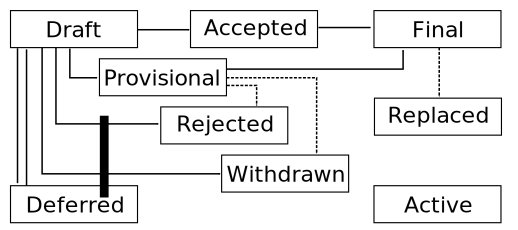
\includegraphics[width=0.9\columnwidth,keepaspectratio]{process-flow} \\[\baselineskip]
        \note[item]{This is the PEP state diagram published in PEP 1. Each state transition represents a potential decision point.}
        \note[item]{This used to have only 8 states. The “provisional” state was added in July 2018 as a consequence of this research.}
        \structurebf{Missing:} the events that occur between states. \tinyskip
        {\tiny (e.g., Draft \(\rightarrow\) \alertbf{? … ?} \(\rightarrow\) Accepted)}
        \note[item]{That is, what happens between these top level states? There’s a lot that can happen between Draft and Accepted! The main problem is that this diagram focuses on the artefacts (PEPs), not the process.}
    \end{center}
\end{frame}


%%%%%%%%%%%%%%%%%%%%%%%%%%%%%%%%%%%%%%%%%%%%%%%%%%%%%%%%%%%%%%%%%%%%%%%%%%%%%%%%


\begin{frame}
    \frametitle{Additional states in the enacted process}
    \framesubtitle{(Savarimuthu et al., 2016; derived from check-in messages)}

    \begin{center}
        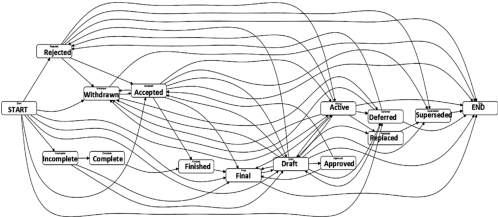
\includegraphics[width=\columnwidth,keepaspectratio]{smitha-states} \\[\baselineskip]
        More states, but finer-grained detail still missing.
    \end{center}
\end{frame}


%%%%%%%%%%%%%%%%%%%%%%%%%%%%%%%%%%%%%%%%%%%%%%%%%%%%%%%%%%%%%%%%%%%%%%%%%%%%%%%%


\begin{frame}
    \frametitle{Stages of the PEP decision-making process}
    \framesubtitle{(manually constructed based on PEP 1 description)}

    \begin{columns}
        \begin{column}{\paperwidth}
            \centering
            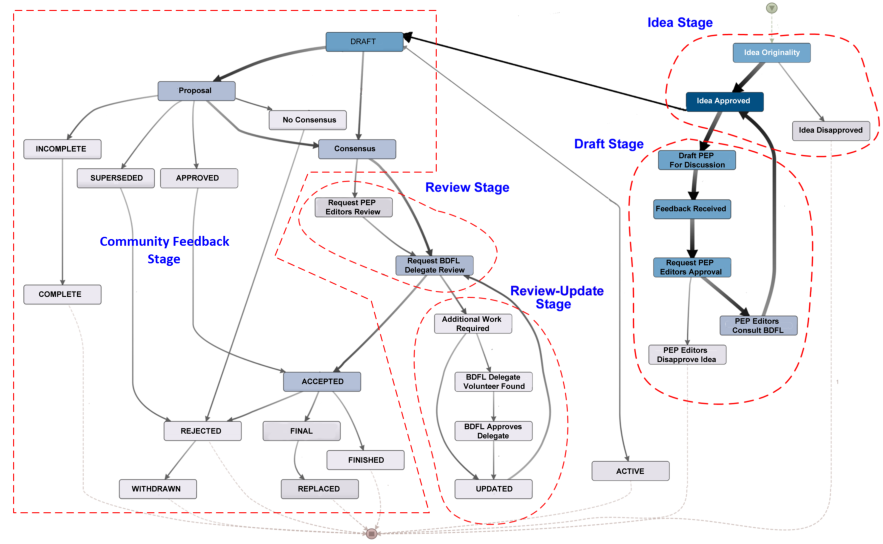
\includegraphics[width=0.9\columnwidth,keepaspectratio]{pep1-process}
            
            But we still don’t have a fully detailed picture (e.g., voting).
            \note[item]{We have at least gained a notion of the different conceptual stages of the process.}
        \end{column}
    \end{columns}
\end{frame}


%%%%%%%%%%%%%%%%%%%%%%%%%%%%%%%%%%%%%%%%%%%%%%%%%%%%%%%%%%%%%%%%%%%%%%%%%%%%%%%%


\begin{frame}
    \frametitle{The data}

    \begin{itemize}
        \item 1,553,564 messages from Python mailing list archives:
        \note[item]{As of the time of writing — we’ve added more recent messages since.}
        \begin{itemize}
            \item April 1999 to October 2018
            \note[item]{There are 7 “rogue” messages from March 1995 that appear to be Linux-related.}
            \item 11 mailing lists \tinyskip
            {\tiny (Python-Dev, Python-Ideas, Python-Commits, Python-Checkins, Python-List, Python-Distutils-Sig,} \tinyskip
            {\tiny Python-Bugs-List, Python-Patches, Python-Announce-Lists, Python-3000, Python-Authors)}
        \end{itemize}
        \item Pre-processing and cleaning:
        \note[item]{Glossing over a lot of detail here.}
        \begin{itemize}
            \item identify messages that explicitly mention one or more PEPs \tinyskip
            {\tiny (by number, e.g., “PEP 123”, or by title, e.g., “PEP Purpose and Guidelines”)}
            \note[item]{Clearly this won’t catch everything, but it’s not bad!}
            \item merge contributors with multiple email addresses
        \end{itemize}
        \item 90,264 unique PEP-related messages covering 467 PEPs. \tinyskip
        {\tiny (63 Informational, 41 Process, 363 Standards Track)}
    \end{itemize}
\end{frame}


%%%%%%%%%%%%%%%%%%%%%%%%%%%%%%%%%%%%%%%%%%%%%%%%%%%%%%%%%%%%%%%%%%%%%%%%%%%%%%%%


\begin{frame}
    \frametitle{Extracting the decision-making process}
    \framesubtitle{(framework)}

    \note[item]{I stole a few figures from Pankaj’s thesis — any issues are his fault \faSmileO.}

    \begin{columns}
        \begin{column}{\paperwidth}
            \centering
            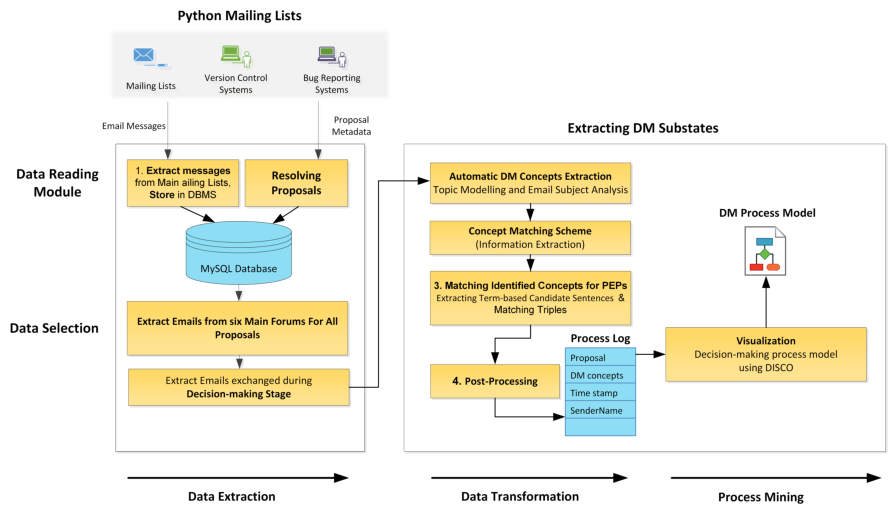
\includegraphics[width=0.95\columnwidth,keepaspectratio]{demap-substates}
        \end{column}
    \end{columns}
\end{frame}


%%%%%%%%%%%%%%%%%%%%%%%%%%%%%%%%%%%%%%%%%%%%%%%%%%%%%%%%%%%%%%%%%%%%%%%%%%%%%%%%


\begin{frame}
    \frametitle{Extracting the decision-making process}
    \framesubtitle{(finding sub-states)}

    \begin{itemize}
        \item Identified 44 decision-making concepts or \emph{sub-states}:
        \begin{itemize}
            \item from literature
            \item from manual analysis of 5642 messages covering 30 PEPs
            \note[item]{21 Standards Track, 5 Informational, 4 Process.}
            \note[item]{We created a custom tool to quickly browse messages related to a specific PEP (next slide).}
        \end{itemize}
        \item Formalised sentences already known to contain these sub-states as 371 unique subject, verb, object (S,V,O) triples. \tinyskip
        {\tiny (using ClausIE)}
        \note[item]{That is, sentences from the 5642 manually examined messages for the 30 PEPs.}
    \end{itemize}
    \medskip

    \begin{columns}
        \begin{column}{\paperwidth}
            \centering
            \resizebox{0.9\columnwidth}{!}{
                \begin{tabular}{llll}
                    \toprule
                    acceptance\_stalled &   co\_bdfl\_delegate\_accepted\_pep   &   member\_volunteers\_bdfl\_delegate  &   positive\_feedback  \\
                    alternative\_pep    &   complementary\_vote     &   member\_willing\_to\_be\_bdfl\_delegate     &   ready\_bdfl\_review     \\
                    approval\_to\_vote  &   complementary\_vote\_results    &   no\_consensus   &   redraft     \\
                    assigned\_pep\_number   &   consensus   &   no\_majority    &   request\_pep\_number    \\
                    bdfl\_asked\_delegate\_volunteer    &   decided\_bdfl\_consensus    &   no\_objections  &   requests\_feedback  \\
                    bdfl\_delegate\_accepted\_pep   &   feedback\_receive   &   not\_enough\_support    &   reviewed    \\
                    bdfl\_delegate\_allocated   &   idea\_approved   &   official\_complementary\_confirm    &   vote    \\
                    bdfl\_delegate\_reviewed    &   idea\_postponed     &   poll    &   vote\_results   \\
                    bdfl\_pronouncement &   idea\_rejected   &   poll\_closed    &   voting\_method\_enquiry     \\
                    bdfl\_pronouncement\_accepted   &   implemented     &   poll\_results   &   voting\_method\_suggestion  \\
                    bdfl\_pronouncement\_rejected   &   lazy\_consensus     &   poll\_results\_no\_majority     &   withdrawn\_by\_author   \\
                    \bottomrule
                \end{tabular}
            }
        \end{column}
    \end{columns}
\end{frame}


%%%%%%%%%%%%%%%%%%%%%%%%%%%%%%%%%%%%%%%%%%%%%%%%%%%%%%%%%%%%%%%%%%%%%%%%%%%%%%%%


\begin{frame}
    \frametitle{Extracting the decision-making process}
    \framesubtitle{(sub-states GUI)}

    \begin{columns}
        \begin{column}{\paperwidth}
            \centering
            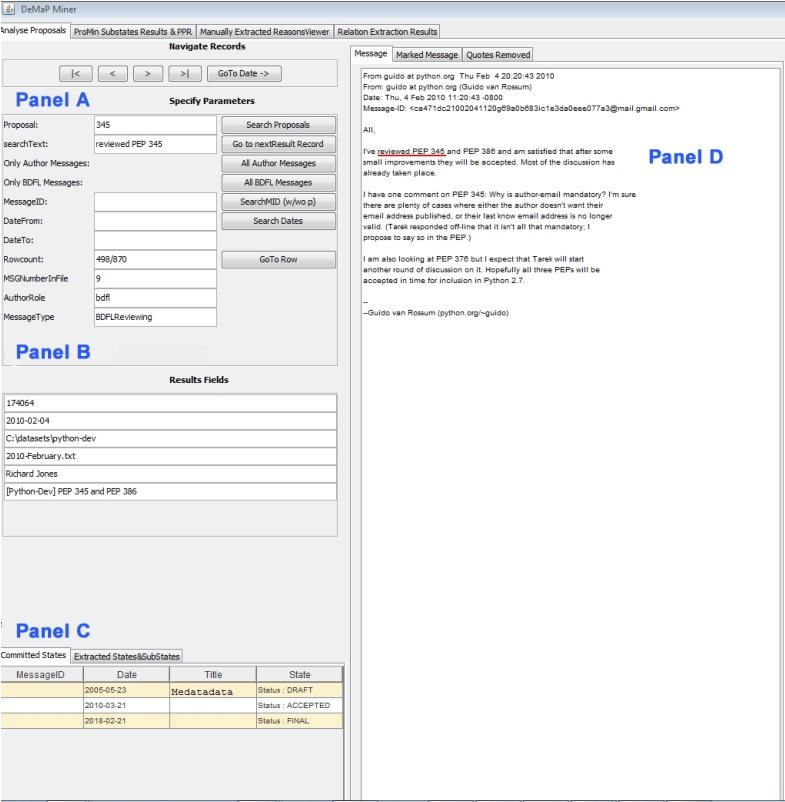
\includegraphics[height=8cm,keepaspectratio]{demap-substates-gui}
        \end{column}
    \end{columns}
    \note[item]{Panel A: search parameters.}
    \note[item]{Panel D: found message(s).}
    \note[item]{Panel B: message metadata.}
    \note[item]{Panel C: top level stage changes for related PEP.}
\end{frame}


%%%%%%%%%%%%%%%%%%%%%%%%%%%%%%%%%%%%%%%%%%%%%%%%%%%%%%%%%%%%%%%%%%%%%%%%%%%%%%%%


\begin{frame}
    \frametitle{Extracting the decision-making process}
    \framesubtitle{(constructing the process diagram)}

    \begin{itemize}
        \item Used automated triple matching to extract candidate sentences from all 90,264 PEP-related messages.
        \item Message timestamp indicated when each sub-state occurred for the corresponding PEP(s).
        \item Sub-state + timestamp data \(\Rightarrow\) DISCO to create process diagrams.
        \item Packaged as a framework called \emph{Decision-Making Process (DeMaP) Miner}.
    \end{itemize}
\end{frame}


%%%%%%%%%%%%%%%%%%%%%%%%%%%%%%%%%%%%%%%%%%%%%%%%%%%%%%%%%%%%%%%%%%%%%%%%%%%%%%%%


\begin{frame}
    \frametitle{Extracted decision-making process for all 467 PEPs}
    \framesubtitle{(summarised: ≈10\% of paths)}

    \begin{columns}
        \begin{column}{\paperwidth}
            \centering
            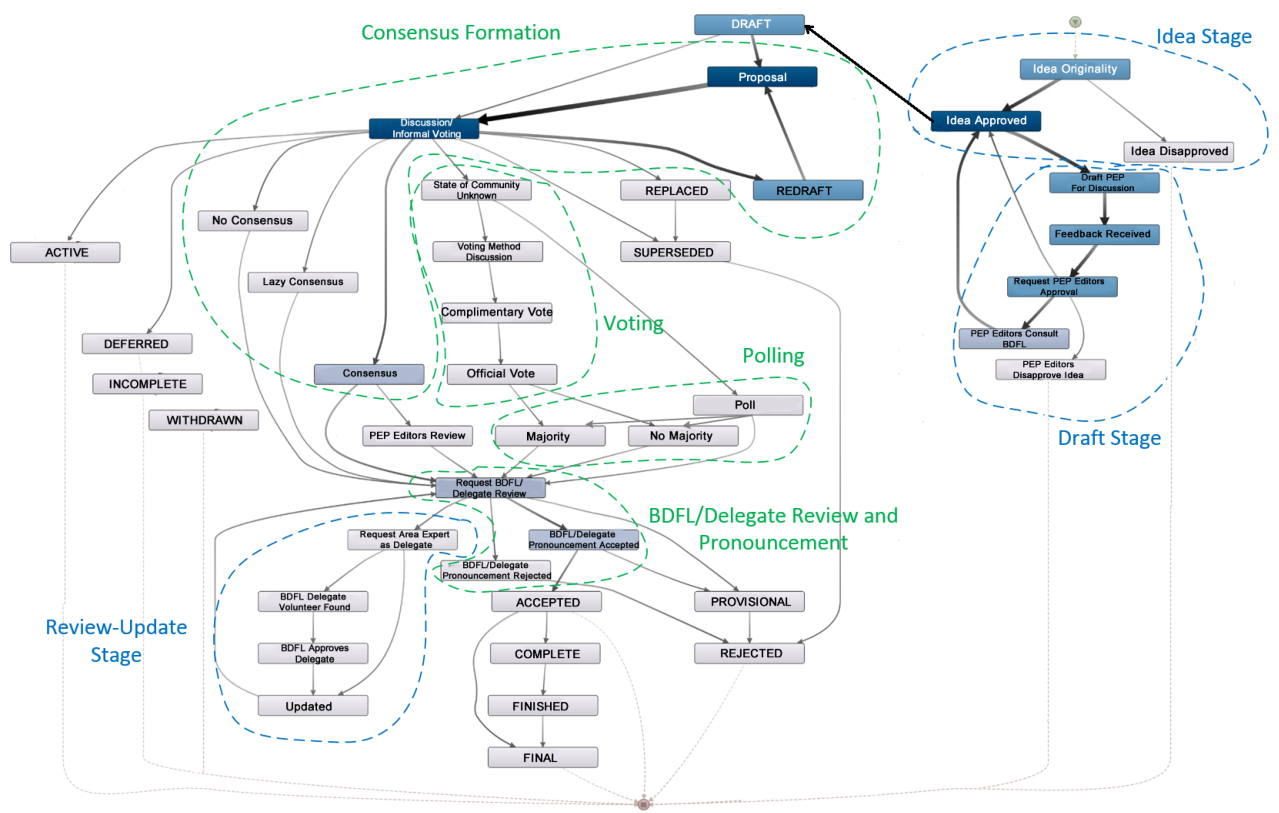
\includegraphics[width=0.95\columnwidth,keepaspectratio]{extracted-process-full}
        \end{column}
    \end{columns}
    \note[item]{Of particular note here are the four additional decision-making activities or stages shown in green, which were not identified elsewhere.}
    \note[item]{The blue activities correspond to the same ones in the manually generated process diagram shown earlier.}
    \note[item]{Interesting things that now clearly appear are the final BDFL decision, and more detail around preference gathering activities (consensus, voting, polling). Also note the redrafting cycle in the consensus formation activity, which wasn’t apparent in the previous models, and the new Provisional top level state.}
    \note[item]{The main differences between polling and voting seem to be around formality of the process and the methods used.}
    \note[item]{Also look at the full version and the PEP type-specific versions on FigShare (paper Section~4.3).}
\end{frame}


%%%%%%%%%%%%%%%%%%%%%%%%%%%%%%%%%%%%%%%%%%%%%%%%%%%%%%%%%%%%%%%%%%%%%%%%%%%%%%%%


\begin{frame}
    \frametitle{Evaluation}

    \begin{itemize}
        \item The three authors manually evaluated 200 random sentences labelled by DeMap Miner:
        \note[item]{Including all the usual inter-rater reliability checking.}
        \note[item]{To confirm that the framework’s performance reasonably well at accurately labelling candidate sentences.}
    \end{itemize}
    \begin{center}
        \footnotesize            
        \begin{tabular}{cccccccc}
            \toprule
            \textbf{TP} & \textbf{TN} & \textbf{FP} & \textbf{FN} & \textbf{Precision} & \textbf{Recall} & \textbf{\emph{F}-score} & \textbf{Accuracy} \\
            121 & 44 & 17 & 18 & 0.88 & 0.87 & 0.87 & 0.82 \\
            \bottomrule
        \end{tabular}
    \end{center}
    \smallskip
    \begin{itemize}
        \item Showed the summarised process diagram to a Python Steering Council member:
        \note[item]{It was during this evaluation that the missing Provisional state was noticed and added to PEP 1.}
    \end{itemize}
    \medskip
    \begin{columns}
        \begin{column}{0.8\columnwidth}
            \emph{“I've now reviewed the diagram, and it looks pretty solid to me, and I think does a good job of capturing the different activities than [sic] can be undertaken through the consensus building phase.”}
        \end{column}
    \end{columns}
\end{frame}


%%%%%%%%%%%%%%%%%%%%%%%%%%%%%%%%%%%%%%%%%%%%%%%%%%%%%%%%%%%%%%%%%%%%%%%%%%%%%%%%


\begin{frame}
    \frametitle{So what?}

    \begin{itemize}
        \item Extracted decision-making process is more complex:
        \begin{itemize}
            \item could reflect evolution over time
            \item makes explicit details missing from earlier models (e.g., BDFL can override community consensus)
            \note[item]{Especially around consensus formation and voting. Overriding consensus is of course implied by the monarchist governance model, but an explicit statement is generally better.}
            \item some differences across PEP types
        \end{itemize}
        \item Benefits of publicising the extracted model: \tinyskip
        {\tiny (but probably not the full diagram! \faSmileO)}
        \begin{itemize}
            \item makes the implicit explicit
            \item beneficial to those “learning the ropes”
        \end{itemize}
        \item DeMaP Miner could potentially be applied to other projects.
    \end{itemize}
\end{frame}


%%%%%%%%%%%%%%%%%%%%%%%%%%%%%%%%%%%%%%%%%%%%%%%%%%%%%%%%%%%%%%%%%%%%%%%%%%%%%%%%


\begin{frame}
    \frametitle{Recent work: Reason extraction}

    \note[item]{I’m not as familiar with this work.}

    \begin{itemize}
        \item What are the reasons behind specific decisions?
        \begin{itemize}
            \item more than just knowing certain sub-states occurred
            \item e.g., what were the critical sub-states leading to a PEP being accepted or rejected?
        \end{itemize}
        \item Heuristics-based decision support system.
    \end{itemize}
\end{frame}


%%%%%%%%%%%%%%%%%%%%%%%%%%%%%%%%%%%%%%%%%%%%%%%%%%%%%%%%%%%%%%%%%%%%%%%%%%%%%%%%


\begin{frame}
    \frametitle{Reason extraction framework}

    \begin{columns}
        \begin{column}{\paperwidth}
            \centering
            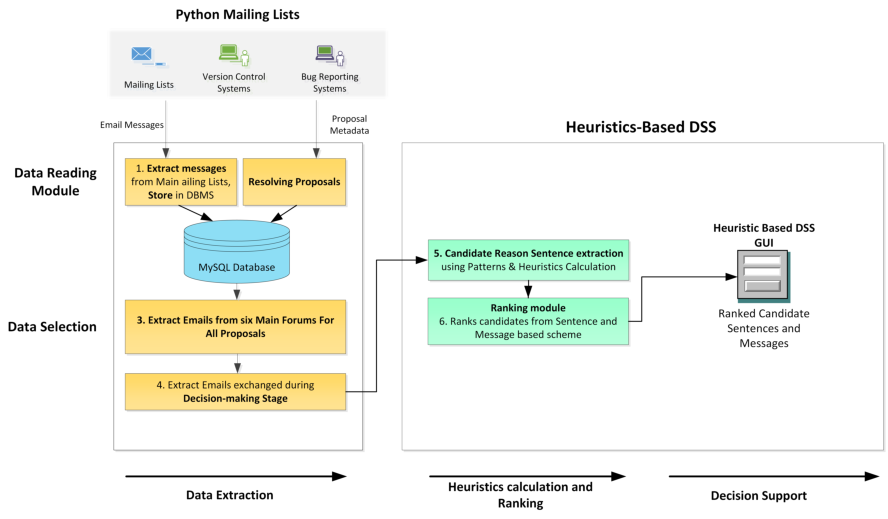
\includegraphics[width=0.95\columnwidth,keepaspectratio]{demap-reasons}
        \end{column}
    \end{columns}
\end{frame}


%%%%%%%%%%%%%%%%%%%%%%%%%%%%%%%%%%%%%%%%%%%%%%%%%%%%%%%%%%%%%%%%%%%%%%%%%%%%%%%%


\begin{frame}
    \frametitle{Reason extraction GUI}

    \begin{columns}
        \begin{column}{\paperwidth}
            \centering
            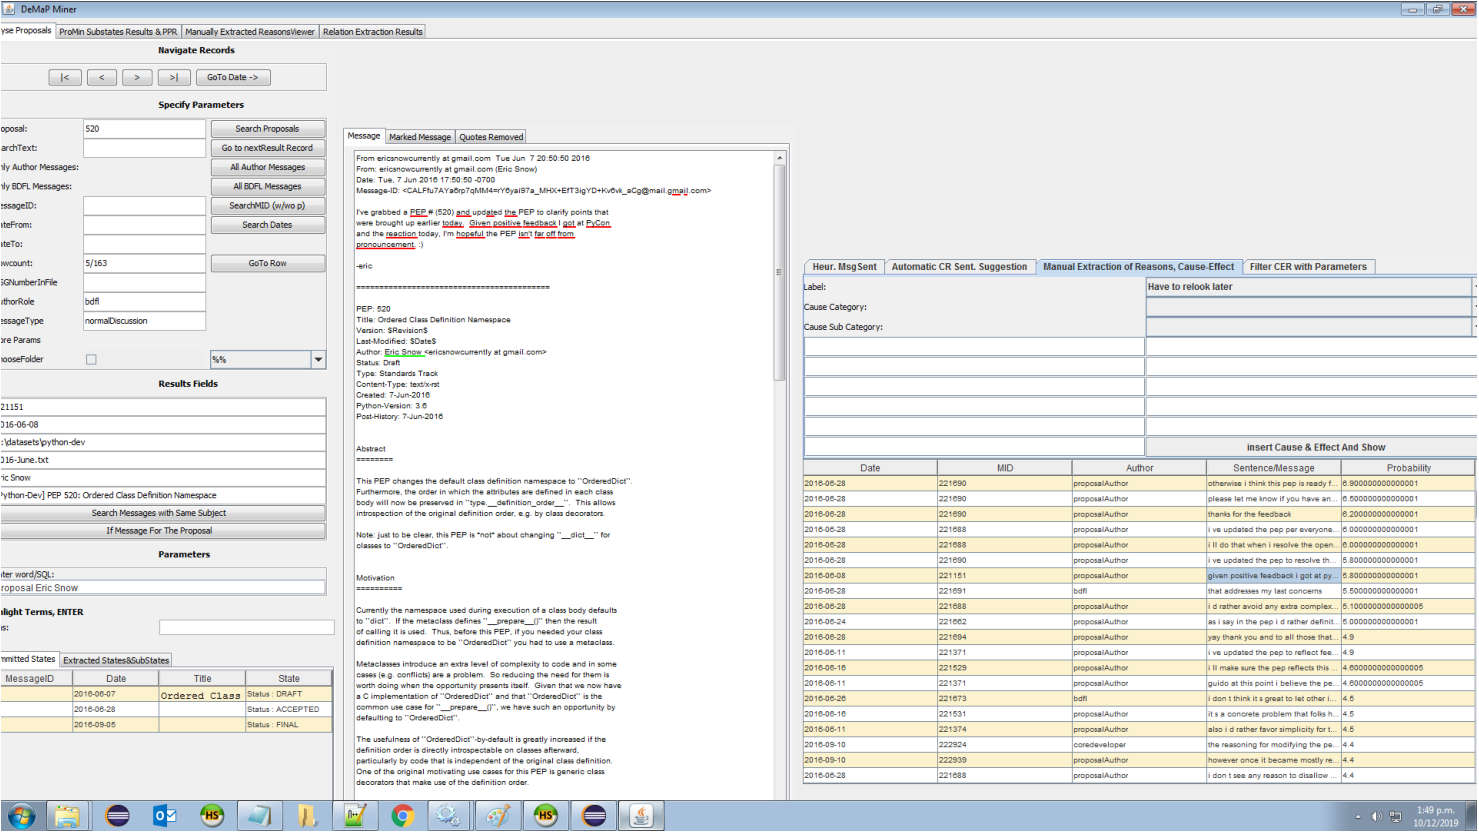
\includegraphics[width=0.98\columnwidth,keepaspectratio]{demap-reasons-gui}
        \end{column}
    \end{columns}
    \note[item]{Left: search parameters (PEP number).}
    \note[item]{Middle: message corresponding to selected reason sentence.}
    \note[item]{Right: ranked candidate reason sentences for current PEP.}
\end{frame}


%%%%%%%%%%%%%%%%%%%%%%%%%%%%%%%%%%%%%%%%%%%%%%%%%%%%%%%%%%%%%%%%%%%%%%%%%%%%%%%%


\begin{frame}
    \frametitle{Ongoing and future work}

    \begin{itemize}
        \item How has Python’s decision-making process evolved over time?
        \note[item]{We have the complete PEP change history (Git), and we can take snapshots of mailing list discussions at different points in time to see how things compare.}
        \item Have things changed under the new governance model?
        \note[item]{Longer term. We might have to wait a couple of years for things to settle in.}
        \item Can we use DeMaP Miner on other OSS projects?
        \begin{itemize}
            \item JCP has a similar process to Python {\tiny (states may differ)}
            \note[item]{So it should be possible to reconfigure DeMaP Miner to work on JEPs without significant reconfiguration.}
            \item only projects with repositories of decision-making discussion
        \end{itemize}
    \end{itemize}
\end{frame}


%%%%%%%%%%%%%%%%%%%%%%%%%%%%%%%%%%%%%%%%%%%%%%%%%%%%%%%%%%%%%%%%%%%%%%%%%%%%%%%%


\begin{frame}
    \frametitle{}

    \begin{center}
        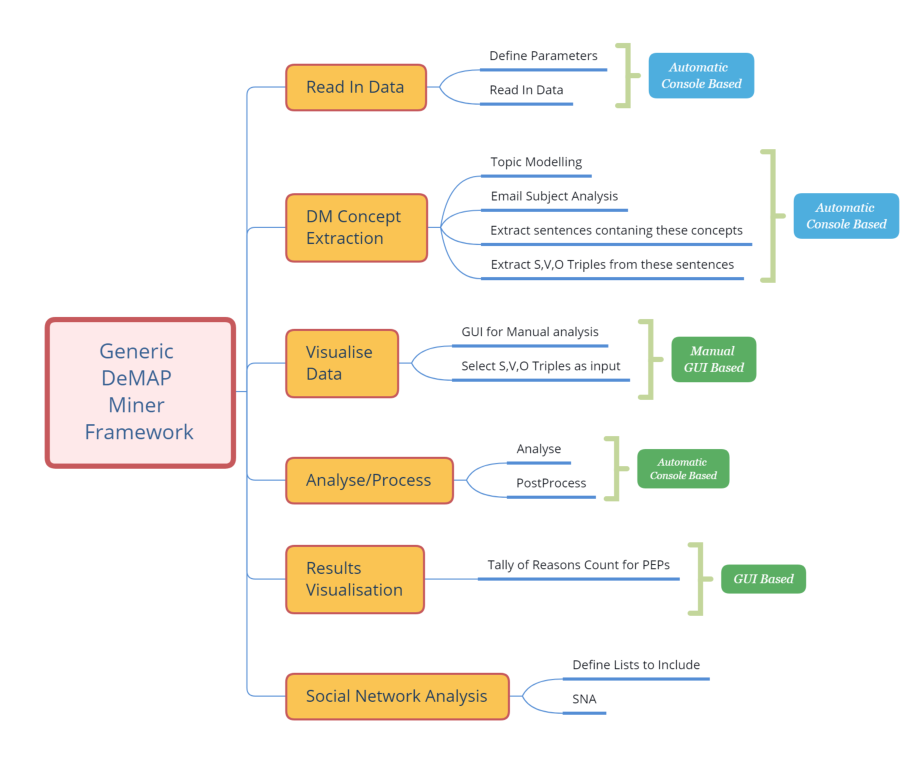
\includegraphics[width=\columnwidth,keepaspectratio]{demap-generic}
    \end{center}
\end{frame}


%%%%%%%%%%%%%%%%%%%%%%%%%%%%%%%%%%%%%%%%%%%%%%%%%%%%%%%%%%%%%%%%%%%%%%%%%%%%%%%%


\begin{frame}
    \centering
    \bigskip
    \bigskip
    {\Huge\structurebf{Thank you}}
    \bigskip

    Questions?
\end{frame}


%%%%%%%%%%%%%%%%%%%%%%%%%%%%%%%%%%%%%%%%%%%%%%%%%%%%%%%%%%%%%%%%%%%%%%%%%%%%%%%%


\end{document}
